%Use one of the two documentclass lines depending on aspect ratio needed
% for 4x3 aspect ratio slides
%\documentclass{beamer}
%for 16x9 (modern wide screen) aspect ratio slides
\documentclass[aspectratio=169]{beamer}
\usepackage[T1]{fontenc}
\usepackage[utf8]{inputenc}
\usepackage{tikz-cd,wrapfig}
\usepackage{tcolorbox}
\usepackage{listings}
\usepackage[export]{adjustbox}
\usepackage[dvipsnames]{xcolor}

% Maths
\usepackage{amsmath}
\usepackage{amssymb}
\usepackage{physics}
\usepackage{siunitx}

% Backup slides
\newcommand{\backupbegin}{
    \newcounter{finalframe}
    \setcounter{finalframe}{\value{framenumber}}
}
\newcommand{\backupend}{
    \setcounter{framenumber}{\value{finalframe}}
}

% Oxford Maths theming
\usetheme{unitnphysics}

% Set author etc info
\title[Bubbles in a ferromagnetic superfluid] %short version of title for slide footer
{Bubbles in a ferromagnetic superfluid} %full title for titlepage
\author{\textbf{Candidate}: Giorgio Micaglio\\\textbf{Supervisor}: dr.\ Alessandro Zenesini}
\institute{Bachelor's Degree in Physics}
\date[March 10, 2025]  %short date for slide footer
{March 10, 2025} %main date for title page,
                        %can overload it to show say 'Conference X, Date Y'


%% Now for the actual slides %%
\begin{document}

\begin{frame}[plain]
  \titlepage
\end{frame}

\begin{frame}{Overview}
  \begin{columns}
      \begin{column}{0.7\textwidth}
          This presentation will cover:
          \begin{itemize}
              \item \textbf{Introduction}
              \item \textbf{Theoretical background}: Ferromagnetism in coherently coupled two-component spin mixtures
              \item \textbf{Data analysis}: Characterization of false vacuum decay bubbles
              \item \textbf{Conclusions}
          \end{itemize}
      \end{column}
      \begin{column}{0.3\textwidth}
          \begin{figure}
              \centering
              \includegraphics[width=\linewidth]{../thesis/figures/chap1/artistic.png}
          \end{figure}
      \end{column}
  \end{columns}
\end{frame}

\begin{frame}{Introduction}
  Why \textbf{bubbles} in a ferromagnetic superfluid?

  ~

  \begin{itemize}
      \item First \textbf{experimental observation} of false vacuum decay (FVD) in the \emph{Pitaevskii BEC Center} laboratories of the University of Trento.
      \item \textbf{Superfluidity}: high degree of coherence of the system
      \item \textbf{Ferromagnetism}: double well energy landscape
      \item Study of FVD provides information on metastability from quantum systems to cosmology
      % \item Framework: \textbf{quantum gas} of Sodium atoms optically trapped and cooled below the condensation temperature
  \end{itemize}
  
\end{frame}

% \section{\textbf{Theoretical background}}

% \begin{frame}{\textbf{Theoretical background}: Ideal Bose gas}
%   The ideal Bose gas is a quantum system of $N$ non-interacting bosons, described by statistical mechanics.
%   \begin{equation*}
%       \langle n_i \rangle = \frac{1}{e^{\beta(\epsilon_i - \mu)}-1}
%   \end{equation*}
%   \onslide<2->
%   The occupation number of the ground state $N_0 = \langle n_0\rangle$ corresponds to the condensation. There is a phase transition at $T = T_c$.
%   \begin{equation*}
%       \frac{N_0}{N} = 1-\left(\frac{T}{T_c}\right)^\alpha \quad \text{for } T < T_c
%   \end{equation*}
%   In a finite box $\alpha = 3/2$, in harmonic confinement $\alpha = 3$.
% \end{frame}

\begin{frame}{Experimental platform}
  \begin{columns}
    \begin{column}{0.5\textwidth}
      \begin{itemize}
        \item $N\sim10^6$ condensed $^{23}$Na atoms in the hyperfine states: 
        \begin{align*}
          &\ket{F,m_F} = \ket{2, -2} = \ket{\uparrow} \\
          &\ket{F,m_F} = \ket{1, -1} = \ket{\downarrow}
        \end{align*}
        \item Contact interaction constants $g_{\uparrow\uparrow}$, $g_{\downarrow\downarrow}$, $g_{\uparrow\downarrow}$
        \item Interconversion due to Rabi coupling: strength $\Omega_R$ and detuning $\delta_B$
        \item Harmonic trapping potential (cigar-shaped, 1D)
        % \item Cooled below the condensation temperature
        % \item Thomas-Fermi radii $R_\perp = 2\ \unit{\micro\meter}$ and $R_x = 200\ \unit{\micro\meter}$ (cigar-shaped)
        % \item Reduction to \textbf{1D system} and spin-selective imaging yield the densities $n_\uparrow(x)$, $n_\downarrow(x)$ and the magnetization $Z(x)$
      \end{itemize}
    \end{column}
    \begin{column}{0.5\textwidth}
      \begin{figure}
        \centering
        \includegraphics[width=\linewidth]{../thesis/figures/chap1/rabi.png}
      \end{figure}
    \end{column}
  \end{columns}
\end{frame}

% \begin{frame}{\textbf{Theoretical background}: Gross-Pitaevskii equation}
%   A system of \textbf{weakly-interacting bosons} can be described by a mean-field approximation with a single wavefunction, yielding the GPE:
%   \begin{equation*}
%       i\hbar \pdv{\psi(x,t)}{t} = \left[ 
%           -\frac{\hbar^2}{2m}\nabla^2 + V(x,t) + g|\psi(x,t)|^2
%       \right] \psi(x,t)
%   \end{equation*}
%   \pause
%   In the stationary case:
%   \begin{equation*}
%       \left[ 
%           -\frac{\hbar^2}{2m}\nabla^2 + V(x) + g|\psi(x)|^2
%       \right] \psi(x) = \mu \psi(x)
%   \end{equation*}
%   When the interaction dominates on the kinetic term:
%   \begin{equation*}
%       n(x) = \frac{\mu - V(x)}{g} \quad \Rightarrow \quad R_{\rm TF} = \sqrt{\frac{2\mu}{m\omega^2}}
%   \end{equation*}
% \end{frame}

\begin{frame}{Coherently coupled two-component spin mixtures}
  The GPEs contain the \colorbox{Dandelion}{intra} and \colorbox{Thistle}{inter}-species interaction constants and the \colorbox{lime}{coupling} between the states:
  \begin{equation*}
    \begin{aligned}
        &\left[ -\frac{\hbar^2}{2m}\nabla^2 + V(x) - \colorbox{lime}{$\dfrac{\delta_B}{2}$} + \colorbox{Dandelion}{$g_{\uparrow\uparrow}$}|\psi_\uparrow(x)|^2 + \colorbox{Thistle}{$g_{\uparrow\downarrow}$}|\psi_\downarrow(x)|^2
        \right] \psi_\uparrow(x) - \colorbox{lime}{$\dfrac{\hbar\Omega_R}{2}$}\psi_\downarrow(x) = \mu_\uparrow \psi_\uparrow(x) \\
        &\left[ -\frac{\hbar^2}{2m}\nabla^2 + V(x) + \colorbox{lime}{$\dfrac{\delta_B}{2}$} + \colorbox{Thistle}{$g_{\uparrow\downarrow}$}|\psi_\uparrow(x)|^2 + \colorbox{Dandelion}{$g_{\downarrow\downarrow}$}|\psi_\downarrow(x)|^2
        \right] \psi_\downarrow(x) - \colorbox{lime}{$\dfrac{\hbar\Omega_R}{2}$}\psi_\uparrow(x) = \mu_\downarrow \psi_\downarrow(x)
    \end{aligned}
  \end{equation*}
  % Depending on the values of $g_{aa}$, $g_{bb}$ and $g_{ab}$, the \textbf{ground state} of the system can behave in different manners
  \pause
  Magnetization $Z = (n_\uparrow-n_\downarrow)/(n_\uparrow+n_\downarrow)$ produces a double well energy landscape:
  \begin{equation*}
      E_{\rm MF}(Z) = -|\delta g|n Z^2 - 2\hbar\Omega_R \sqrt{1-Z^2} - 2\hbar\delta_{\rm eff} Z
      \label{eq:E_MF}
  \end{equation*}
\end{frame}

\begin{frame}{Magnetic model phase diagram: para and ferro}
  \begin{minipage}{0.7\textwidth}
    \begin{figure}
      \centering
      \includegraphics[width=\linewidth]{images/ferro.png}
    \end{figure} 
  \end{minipage}
  \hspace{0.01\textwidth}
  \begin{minipage}{0.27\textwidth}
    \begin{itemize}
      \item Set $\dfrac{|\delta g| n}{\hbar\Omega_R}$ to a fixed value by adjusting $\Omega_R$
      \item Probe the magnetic properties by changing $\delta_{\rm eff}$
    \end{itemize}
  \end{minipage}
\end{frame} 

\begin{frame}{False vacuum decay bubbles}
  \begin{minipage}{0.32\textwidth}
    \begin{itemize}
      \item Quantum tunnelling from A to B (stochastic)
      \item Decay from B to C (what we want to study)
      \item Problem: when to take the shot?
    \end{itemize}
  \end{minipage}
  \hspace{0.01\textwidth}
  \begin{minipage}{0.65\textwidth}
    \begin{figure}
      \centering
      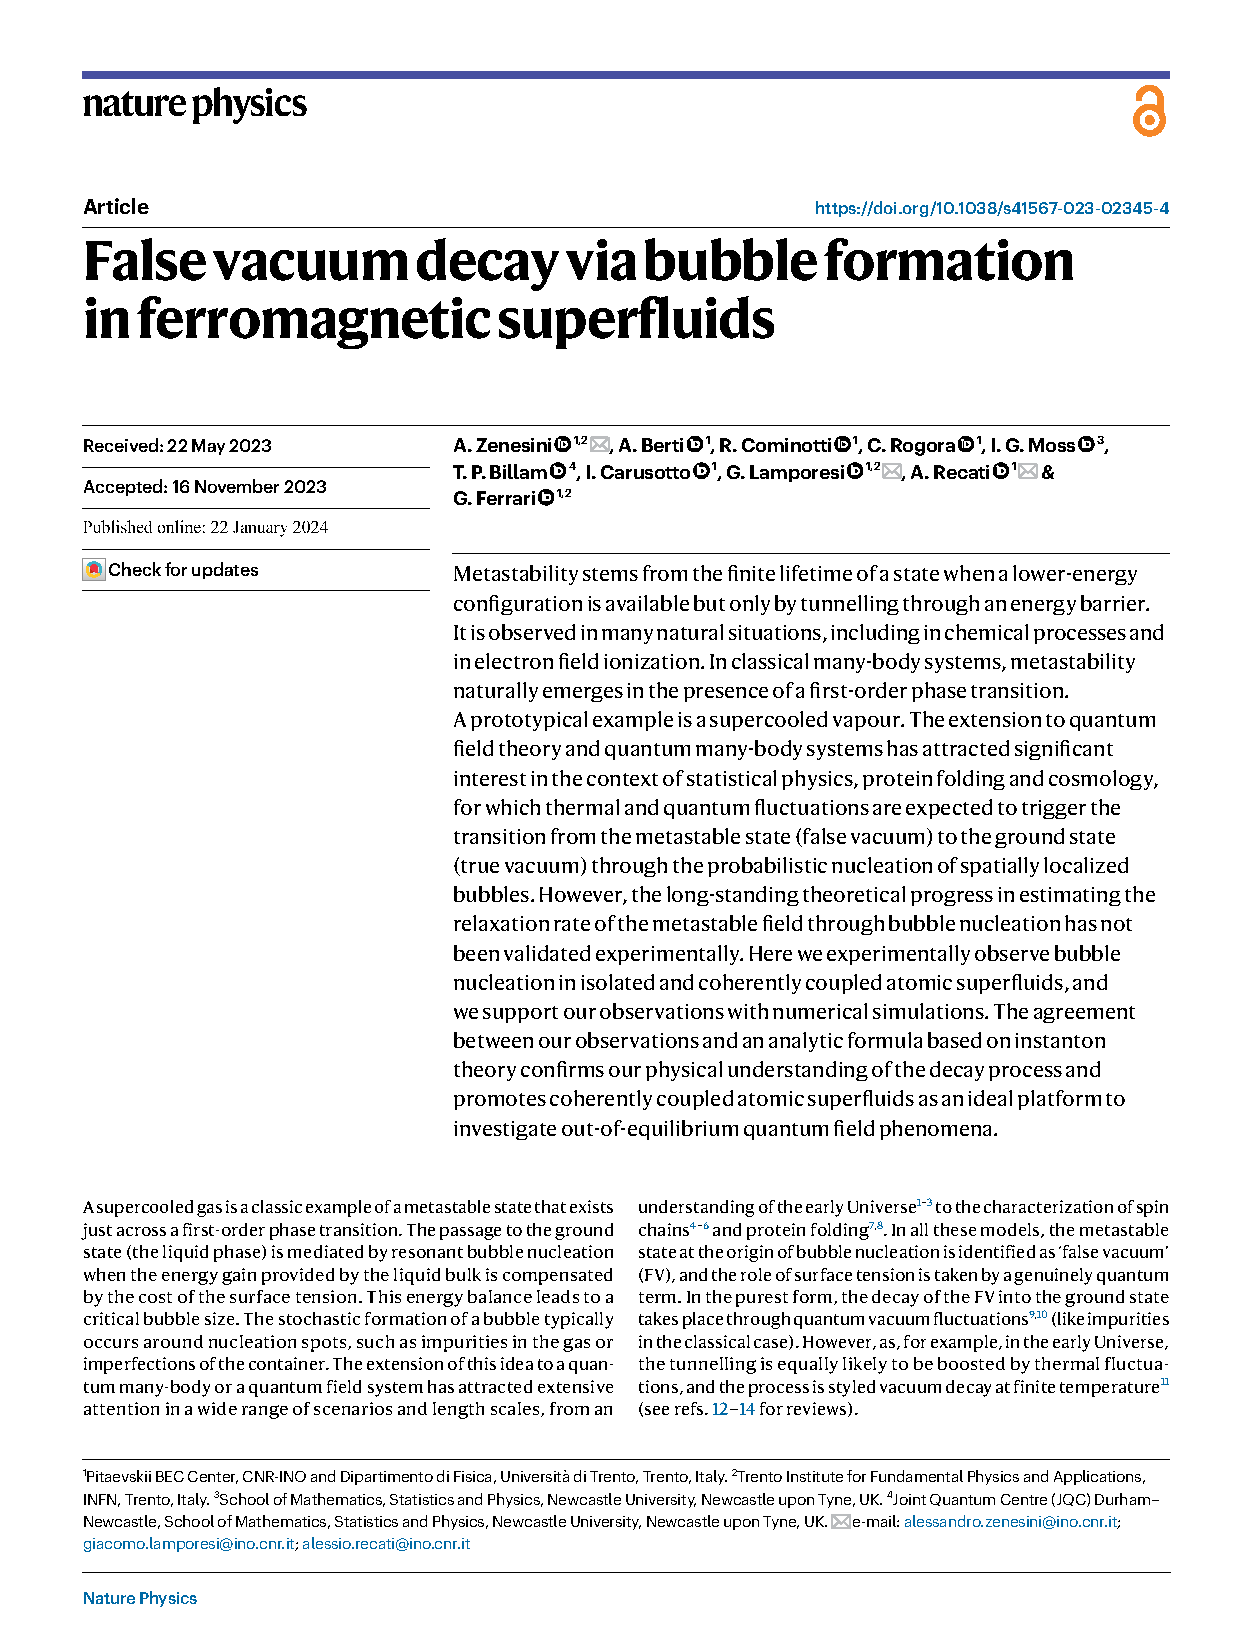
\includegraphics[width=\linewidth]{../thesis/figures/chap1/FVD.png}
    \end{figure} 
  \end{minipage}
\end{frame}

\begin{frame}{Example of bubble shots}
  \begin{figure}
    \centering
    \includegraphics[width=\textwidth]{images/two_bubbles.png}
  \end{figure}
  Our aim is to study:
  \begin{itemize}
    \item Size $\sigma_B$ and domain wall width $w_D$
    \item Excitation structures inside/outside
  \end{itemize}
\end{frame}

\begin{frame}{Bubble fitting routines}
  \begin{figure}
      \centering
      \includegraphics[width=\textwidth]{../thesis/figures/chap2/arctan_fit.png}
  \end{figure}
\end{frame}

\begin{frame}{Shot sorting}
  \begin{figure}
      \centering
      \includegraphics[width=0.9\textwidth]{../thesis/figures/chap2/shot_sorting.png}
  \end{figure}
\end{frame}

\begin{frame}{Analysis of domain wall width and bubble size}
  \begin{minipage}{0.70\textwidth}
    % \vspace{-0.05cm}
    \begin{figure}
        \centering
        \includegraphics[width=\linewidth]{images/b_param_cluster.png}
    \end{figure}
  \end{minipage}
  \hspace{0.01\textwidth}
  \begin{minipage}{0.27\textwidth}
    \begin{itemize}
      \item Shots clustered by size (left) or time (right)
      \item Fit function:
      \[
        \sigma_B(t) = A\left(\frac{t}{1\ \unit{\milli\second}}\right)^B
      \] 
    \end{itemize} 
  \end{minipage}
\end{frame}

\begin{frame}{Spectral analysis in the inside region}
  \begin{columns}
    \begin{column}{0.7\textwidth}
      \begin{figure}
        \centering
        \includegraphics[width=\linewidth]{../thesis/figures/chap2/inside_omdet.png}
      \end{figure}
    \end{column}
    \begin{column}{0.3\textwidth}
      \hspace{-0.2\textheight}
      \begin{figure}
        \centering
        \includegraphics[width=\linewidth]{images/inside_arr.png}
      \end{figure}
      \hspace{0.2\textheight}
      \begin{itemize}
        \item FFT: broad peak at $k \sim 0.01$ \unit{\per\micro\meter}
        \item ACF: peak at $\Delta x \sim 11$ \unit{\micro\meter}
      \end{itemize}
    \end{column}
  \end{columns}
  
\end{frame}

% \begin{frame}{\textbf{Data analysis}: FFT and ACF}
%   \begin{figure}
%       \centering
%       \includegraphics[width=0.8\textwidth]{../thesis/figures/chap2/inside_fft_avg.png}
%   \end{figure}
% \end{frame}

\begin{frame}{ACF analysis in the inside region vs $\sigma_B$ (fits)}
  \begin{columns}
    \begin{column}{0.50\textwidth}
      \begin{figure}
        \centering
        \adjincludegraphics[width=\linewidth, trim={0 0 {.5\width} 0}, clip]{../thesis/figures/chap2/fit_size_inside.png}
      \end{figure}
    \end{column}
    \begin{column}{0.50\textwidth}
      \begin{figure}
        \centering
        \includegraphics[width=\linewidth]{images/inside_arr.png}
      \end{figure}
      \begin{itemize}
        \item Shots clustered by increasing size (darker to lighter colors)
        \item Fit function $\mathcal{A}_{\rm fit}(x) = $
        \begin{equation*}
          (1 - \Delta)\cos(\frac{\pi x}{\ell_2})\exp[-\frac{1}{2}\left(\frac{x}{\ell_1}\right)^{1.7}] + \Delta
        \end{equation*}
      \end{itemize}
    \end{column}
  \end{columns}
\end{frame}

\begin{frame}{ACF analysis in the inside region vs $\sigma_B$ (parameters)}
  \begin{columns}
    \begin{column}{0.7\textwidth}
      \begin{figure}
        \centering
        \includegraphics[width=\linewidth]{images/param_size_inside.png}
      \end{figure}
    \end{column}
    \begin{column}{0.3\textwidth}
      Healing lengths:
      \begin{align*}
        &\xi_s = \frac{\hbar}{\sqrt{2mn|\delta g|}} \approx 0.5\ \unit{\micro\meter}\\
        &\xi_d = \frac{\hbar}{\sqrt{2mn\overline{g}}} \approx 0.01\ \unit{\micro\meter}\\
        &\xi_R = \sqrt{\frac{\hbar}{m\Omega_R}} \approx \numrange[range-phrase=-]{1.8}{3.0}\ \unit{\micro\meter}
      \end{align*}
    \end{column}
  \end{columns}
\end{frame}

\begin{frame}{ACF analysis in the inside region vs $\Omega_R$ (fit and parameters)}
  \begin{figure}
      \centering
      \includegraphics[width=0.9\textwidth]{images/fit_omega_inside.png}
  \end{figure}
\end{frame}

\begin{frame}{ACF analysis in the outside region vs $\sigma_B$ (fits)}
  \begin{columns}
    \begin{column}{0.55\textwidth}
      \begin{figure}
        \centering
        \adjincludegraphics[width=\linewidth, trim={{.5\width} 0 0 0}, clip]{../thesis/figures/chap2/fit_size_outside.png}
      \end{figure}
    \end{column}
    \begin{column}{0.45\textwidth}
      \begin{figure}
        \centering
        \includegraphics[width=\linewidth]{images/outside_arr.png}
      \end{figure}
      \begin{itemize}
        \item Shots clustered by increasing size (darker to lighter colors)
        \item Fit function:
        \[
          \mathcal{A}_{\rm fit}(x) = (1-\Delta)\exp[-\frac{x}{2\ell_1}] + \Delta
        \]
      \end{itemize}
    \end{column}
  \end{columns}
\end{frame}

\begin{frame}{ACF analysis in the outside region vs $\sigma_B$ and $\Omega_R$}
  \begin{columns}
    \begin{column}{0.5\textwidth}
      \begin{figure}
        \centering
        \includegraphics[width=\linewidth]{images/param_size_outside.png}
      \end{figure}
    \end{column}
    \begin{column}{0.5\textwidth}
      \begin{figure}
        \centering
        \includegraphics[width=\linewidth]{images/fit_omega_outside.png}
      \end{figure}
    \end{column}
  \end{columns}
\end{frame}

\begin{frame}{Conclusions}
  What did we learn?
  \begin{itemize}
    \item System shows \textbf{different properties} between inside and outside of the bubble
    \item Domain wall width \textbf{depends on the coupling} strength $\Omega_R$
    \item Growth factor of the bubble size in time is \textbf{independent} of $\Omega_R$
    \item In the bubble, periodic structures \textbf{disappear} with size increasing. They \textbf{appear}, instead, outside of the bubble.
    \item Length scale of information outside is related to the Rabi \textbf{healing length}
  \end{itemize}
  \pause
  Future research:
  \begin{itemize}
    \item Analysis of the \textbf{density} channel
    \item Comparison with numerical GPE \textbf{simulations}
    \item Behavior at different \textbf{temperatures}
  \end{itemize}
\end{frame}

\begin{frame}
  \huge
  Thank you for your attention!
\end{frame}

% \backupbegin
% \begin{frame}
  
% \end{frame}
% \backupend

\end{document}
